\documentclass[11pt,oneside,openany]{book}
\usepackage{bespoke}
\hypersetup{pdftitle={Bespoke: project report},pdfauthor={Ritesh Roshan}}

\begin{document}
\frontmatter
\pagestyle{empty}

\begin{titlepage}
\centering
\vspace*{38mm}
{\fontsize{40}{44}\selectfont\scshape bespoke\par}
\vspace{12mm}
{\Large Clothes made from your words:\\[3pt] a customer's description and pictures turned into a garment a tailor can cut\par}
\vspace{16mm}
{\large\itshape Project report\par}
\vspace{4mm}
{\normalsize\color{soft} Text Analytics and Big Data Analytics\par}
\vfill
{\large Ritesh Roshan\par}
\vspace{12mm}
{\normalsize Amrita School of Artificial Intelligence, Faridabad\par}
\vspace{3mm}
{\normalsize\color{soft} October 2026\par}
\vspace*{14mm}
\end{titlepage}

\chapter*{Summary}
\pagestyle{body}
Most custom clothing in India is ordered through chat messages and phone photos. What reaches the cutting table is the tailor's memory of that conversation. Bespoke replaces the memory with a specification. A customer types or speaks a request in English, Hinglish or Hindi, answers a few questions by tapping pictures, and receives a tailor sheet in English and Hindi, searches for ready-made alternatives, and fabric to buy.

The system is built and deployed. Its language engine runs entirely in the browser: a gazetteer over an ontology of 1,212 surface forms and 47 garment types, a fine-tuned 33-million-parameter MiniLM token classifier exported to 33.8\,MB of int8 ONNX, a constrained Viterbi decoder, a binder that attaches values to garment parts, and a state tracker that folds every turn into a versioned design. On 52 held-out hand-written requests the deployed tagger reaches span F1 of 0.953 (95\% interval 0.918 to 0.982), ahead of rules (0.936), a CRF (0.900) and an HMM (0.751). An answer appears 75\,ms after the customer presses send (median; 130\,ms at the 95th percentile). An optional language-model layer on a serverless function handles what the engine cannot, and every value it returns is checked against the ontology before it is used.

Choices are made by looking. A pipeline generates a library of 171 line drawings and photographs, one for each ontology value, on a 6\,GB laptop GPU with FLUX.2 [klein] 4B (Apache 2.0), ranks them with CLIP for review by hand, and serves them as static files; the library is being generated as this report is written. The application is covered by seven kinds of tests, from 352 parity fixtures between the Python and browser engines to accessibility audits in a real browser. This report describes the workflow, the models, the measurements and what remains.

\cleardoublepage
\tableofcontents

\mainmatter
\pagestyle{body}
\chapter{Introduction}

\section{The problem}
About 12 million people in India work as custom tailors \cite{dataforindia}. Their customers describe what they want in a mixture of English, Hindi and the two together: ``kurti chahiye, fitted at the waist, neeche se thoda loose, V neck thoda deep''. They send screenshots from Instagram and Pinterest and circle the parts they like. The tailor reads all of it, asks a few questions on the phone, and cuts. Nothing in this chain is written down in a form the tailor can check against. When the garment comes back wrong, there is no record of what was asked for.

Software for fashion understands product titles and catalogue images well. It does not take a customer's loose description, find which part of the garment each word is about, notice what is still missing, ask about it in the order that matters to a tailor, and hand over a sheet the tailor can cut from. The research plan that preceded this work reviewed fifteen papers from 2022 to 2026 and found that the closest systems take one clean input, ignore code-mixed language and Indian garments, and never ask a question \cite{bian2025chatgarment,cheng2026chatpref}.

\section{What was built}
Bespoke is a web application with one job: from what a customer says and shows, produce a garment specification and a tailor sheet. It has five views.

\begin{description}[leftmargin=0pt,labelsep=0.6em,itemsep=4pt,font=\normalfont\scshape]
\item[Home] explains the service and starts a design.
\item[Talk] is the conversation. The customer types or speaks; the assistant restates the design in one sentence, lists what it understood on an order card beside the conversation, and asks at most two questions, answered by tapping pictures.
\item[Board] is a moodboard on an embedded Excalidraw canvas. Pictures, notes and arrows are read together; words always outrank pictures.
\item[Sheet] is the tailor sheet in English or Hindi, with drawings of the chosen neckline, sleeves, shape and length, measurements and the finished sizes they imply.
\item[Shop] turns the design into searches on Indian stores, Pinterest boards for ideas, fabric by the metre and tailors nearby.
\end{description}

\section{Contributions}
\begin{enumerate}
\item A complete language engine for garment requests that runs in the browser with no server: ontology, gazetteer, fine-tuned transformer tagger, constrained decoding, part binding and turn-by-turn state, measured against hand-written requests with confidence intervals.
\item A ladder of tagging methods taught in the course (rules, HMM, CRF, transformer), trained and tested on the same split, so each step's gain is visible.
\item A question policy that asks only what a tailor needs for this kind of garment, ordered by the cost of a wrong guess.
\item A visual picker: a pipeline that makes 171 pictures, one per ontology value, on a laptop GPU with an open model, ranks them automatically for review by hand, and serves them so customers choose by looking.
\item A deployed application with an optional language-model layer whose output is validated against the ontology, and a test suite that covers unit, regression, functional, integration, smoke, usability, edge-case and latency testing.
\end{enumerate}

\section{How the course maps onto the work}
From Text Analytics: tokenisation and normalisation of code-mixed text, gazetteers and collocations, sequence labelling with HMMs and CRFs, the Viterbi algorithm, transformer encoders and transfer learning, evaluation with precision, recall, F1 and bootstrap intervals, and speech recognition as an input channel. From Big Data Analytics: the weak-label corpus is generated from the 44,000-row Myntra catalogue \cite{aggarwal2019myntra}, the ontology is the schema shared by every component, and the data platform described in the plan (Spark over public retail data and the order log) is the next phase; Chapter~\ref{ch:phases} states what is built and what is not.

\section{Structure of this report}
Chapter~\ref{ch:system} gives the workflow from a sentence to a tailor sheet. Chapter~\ref{ch:language} describes the language engine and its ladder of models. Chapter~\ref{ch:pictures} describes how the picture library was made. Chapter~\ref{ch:app} covers the application and its deployment, Chapter~\ref{ch:tests} the tests and measurements, Chapter~\ref{ch:phases} the phases, and Chapter~\ref{ch:end} the limits and what comes next.

\chapter{System and workflow}\label{ch:system}

\section{From a sentence to a tailor sheet}
Figure~\ref{fig:system} shows the whole system. Everything inside the shaded region runs in the customer's browser. The page loads the ontology and the engine as code, downloads the 33.8\,MB tagger once and keeps it in the browser cache, and from then on understands a request without a network call. Two things live outside: an optional language-model layer on a serverless function, and the picture library, which is a folder of static files.

\begin{figure}[tbp]
\centering
\resizebox{\linewidth}{!}{\begin{tikzpicture}[x=1cm,y=1cm,
  n/.style={text width=2.6cm,font=\small,inner ysep=5pt,minimum height=1.35cm},
  s/.style={font=\scriptsize,text=soft}]
% row 1: words through the engine
\node[blue,n] (say) at (0,0) {words\\{\footnotesize\color{soft}typed or spoken}};
\node[lav,n] (norm) at (3.4,0) {normalise\\{\footnotesize\color{soft}tokens, spelling by sound}};
\node[lav,n] (tag) at (6.8,0) {tag spans\\{\footnotesize\color{soft}gazetteer, then MiniLM}};
\node[lav,n] (bind) at (10.2,0) {bind\\{\footnotesize\color{soft}parts, sets, seasons, negation}};
\node[rose,n,planned] (llm) at (13.8,-1.3) {model layer\\{\footnotesize\color{soft}optional, serverless}};
% row 2: pictures and the design
\node[peach,n] (board) at (0,-2.6) {moodboard\\{\footnotesize\color{soft}pictures, notes, arrows}};
\node[peach,n] (read) at (3.4,-2.6) {read the board\\{\footnotesize\color{soft}CLIP, pooled, capped}};
\node[green,n] (spec) at (10.2,-2.6) {DesignSpec $v_k$\\{\footnotesize\color{soft}a fold of updates}};
% row 3: what the customer gets
\node[grey,n] (shop) at (6.8,-5.2) {shop\\{\footnotesize\color{soft}stores, Pinterest, fabric, tailors}};
\node[sand,n] (sheet) at (10.2,-5.2) {tailor sheet\\{\footnotesize\color{soft}English or Hindi, with drawings}};
\node[blue,n] (ask) at (13.8,-5.2) {reply\\{\footnotesize\color{soft}one sentence, two questions by picture}};
\node[grey,n] (lib) at (13.8,-7.6) {picture library\\{\footnotesize\color{soft}171 static files}};
\draw[flow] (say) -- (norm);
\draw[flow] (norm) -- (tag);
\draw[flow] (tag) -- (bind);
\draw[flow] (board) -- (read);
\draw[flow] (bind) -- (spec);
\draw[flow] ([yshift=3mm]read.east) -- ([yshift=3mm]read.east-|spec.west);
\draw[flow] ([yshift=-3mm]spec.west) -| (shop.north);
\draw[flow] (spec) -- (sheet);
\draw[flow] (spec.east) -| (ask.north);
\draw[dflow] (lib) -- (ask);
\draw[dflow] (say.north) -- ++(0,0.75) -| node[pos=0.25,above,s]{the same message, in parallel} ([xshift=5mm]llm.north);
\draw[dflow] ([xshift=-5mm]llm.north) |- node[pos=0.25,right,s,align=left]{checked against\\the ontology} (bind.east);
\draw[dflow] (ask.west) -- ++(-0.45,0) |- node[pos=0.25,left,s,align=right]{answers\\fold back} ([yshift=-3mm]spec.east);
\begin{scope}[on background layer]
\node[group,draw=lavD,fill=lavF!25,fit=(norm)(tag)(bind)(read)(spec),inner sep=8pt] (br) {};
\end{scope}
\node[gtitle,text=lavT,anchor=south] at (5.6,-3.5) {in the browser};
\end{tikzpicture}
}
\caption{The system as deployed. The shaded blocks run in the customer's browser on every request. The dashed model layer runs only when a key is configured, in parallel with the engine, and its output is checked against the ontology before it reaches the design. Answers given by tapping a picture fold back into the design as updates.}
\label{fig:system}
\end{figure}

A turn has five steps (Figure~\ref{fig:turn}). The words are normalised: lower-cased, tokenised, and corrected where a word is close in sound to a known garment term (``kurtee'' becomes kurti, ``pass del'' becomes pastel), guarded by the tagger's vocabulary so that ordinary words are left alone. The tagger marks spans with one of 21 types. The binder turns spans into updates on named slots, attaching each value to the part it describes and resolving sets (a top and a bottom named together become a co-ord set) and seasons (``in the cold'' becomes winter, which changes the fabric question). The updates are folded into the design. The question policy then picks what to ask.

\begin{figure}[tbp]
\centering
\resizebox{\linewidth}{!}{\begin{tikzpicture}[x=1cm,y=1cm,
  st/.style={box,text width=2.35cm,font=\footnotesize,minimum height=3.15cm,align=left,anchor=north},
  hd/.style={font=\small\scshape,anchor=base},
  nb/.style={font=\scriptsize,text=soft,anchor=base}]
\def\dx{3.3}
\foreach \i/\h/\f/\d/\t in {
 0/{1 words}/blueF/blueD/{``i want a sweatshirt and pants dark blue cord set that i can wear in the cold''},
 1/{2 spans}/lavF/lavD/{\textsc{garment} sweatshirt, pants\\\textsc{shade} dark\\\textsc{colour} blue\\\textsc{garment} cord set\\\textsc{occasion} cold},
 2/{3 bound}/lavF/lavD/{garment: co-ord set\\pieces: sweatshirt, pants\\colour: navy\\season: winter},
 3/{4 design}/greenF/greenD/{DesignSpec version 1, each value with its source and confidence},
 4/{5 asked}/sandF/sandD/{How should the top fit?\\Which fabric? Warm ones: fleece, wool, terry}}{
  \node[hd] at (\i*\dx,0.45) {\h};
  \node[st,fill=\f,draw=\d] (s\i) at (\i*\dx,0) {\t};
}
\foreach \a/\b in {0/1,1/2,2/3,3/4}{\draw[flow] (s\a.east) -- (s\b.west);}
\node[nb] at (0*\dx,-3.4) {typed, or Whisper};
\node[nb] at (1*\dx,-3.4) {0.05 to 20 ms};
\node[nb] at (2*\dx,-3.4) {sets and seasons};
\node[nb] at (3*\dx,-3.4) {a fold of updates};
\node[nb] at (4*\dx,-3.4) {no neckline question};
\end{tikzpicture}
}
\caption{One turn on a real request that the first version of the system got wrong. It now becomes a navy co-ord set for winter, and the assistant asks about fit and warm fabrics rather than a neckline.}
\label{fig:turn}
\end{figure}

\section{The design as a fold}
The design is never edited in place. Every source of evidence (the words, a picture, an answer, an edit on the order card) produces a list of updates, and the design is the result of applying them in order:
\[
\mathrm{spec}_k = \mathrm{apply}(\mathrm{spec}_{k-1},\; u_1, u_2, \dots, u_n), \qquad u_i \in \{\textsc{set}, \textsc{add}, \textsc{exclude}, \textsc{replace}, \textsc{compare}, \textsc{note}\}.
\]
Each value carries its source and a confidence $p$. Sources are ranked: an edit on the order card outranks an answer to a question, which outranks the customer's words, which outrank a note on the board, a picture and the stored profile. A later update replaces an earlier one when its source ranks at least as high, or when it is more confident by more than 0.25, so a guess from a picture never overwrites something the customer said. An exclusion (``no heavy work'', ``not too flashy'') removes the value and stops it coming back. A comparison (``deeper than picture 2'') is kept until the board is read and then resolved against the picture. Because the design is a fold, every version can be rebuilt, the order card can show where each value came from, and the tailor sheet can mark which instructions were the customer's words and which were defaults.

\section{Which questions to ask}
A tailor needs different things for different garments. The ontology groups the 47 garments into seven families (long tops, short tops, knits, outerwear, bottoms, sets and drapes) and lists, for each family, the slots that must be settled. A slot is asked about when it is missing or its confidence is below 0.7, and slots are ordered by
\[
\mathrm{priority}(s) = \mathrm{cost}(s)\,\bigl(1 - p(s)\bigr),
\]
where the cost is how expensive a wrong guess is at the cutting table. A neckline cut too deep cannot be raised, so neckline depth costs 9; colour costs 4. The options offered depend on the garment as well: a sweatshirt is asked about crew, hood, turtle or V necks and about regular, relaxed or oversized fit; a kurti about round, V, boat, square, sweetheart or mandarin necklines and about fit at the bust and waist. When nothing is left to ask, the conversation ends with the tailor sheet, ideas and shopping in place.

\chapter{The language engine}\label{ch:language}

\section{The ontology}
Every component shares one file, the ontology. It names 21 span types (garment, part, fit, silhouette, length, neckline, sleeve, colour, shade, fabric, pattern, finish, occasion, style, and the small words that change meaning: intensity, negation, comparison, location, dimension, number and reference), 1,212 surface forms that map to canonical values, 47 garment types in seven families, the 18 slots of a design with the cost of getting each wrong, the questions each family needs, fabrics suited to each season, and the Hindi term for every value so that the tailor sheet can be printed in Hindi. Forms include Hinglish and Devanagari spellings (\hi{कुर्ती}, kurta, kurtee), so ``lehenga chahiye shaadi ke liye, maroon, gota patti'' is read without translation. The Python engine used for training and the TypeScript engine in the browser both load this file, and 352 fixtures check that they agree.

\section{Data}
There is no public corpus of customers describing garments to tailors, so the training data is weakly labelled and the test data is written by hand.

\paragraph{Training} 12,000 sentences: 8,000 generated from clause templates that combine attribute bags in random order with distractor phrases, so the model cannot learn position, and 4,000 product titles from the Myntra catalogue of 44,000 items \cite{aggarwal2019myntra}, labelled by the gazetteer. A further 1,000 generated sentences are used to choose the checkpoint.

\paragraph{Evaluation} 82 requests written by hand in bracket markup, in the way customers write: run-on, misspelt, mixing languages. The first 30 are a development set; the remaining 52 are the test set and were not looked at while building the engine. Seven labels were changed when the ontology grew to version 1.1, and each change is recorded. The set is small, so every result is reported with a 95\% bootstrap interval over requests.

\section{A ladder of taggers}
Each method taught in the course was trained on the same data and scored on the same 52 requests (Figure~\ref{fig:ladder}). Spans count as correct only when both boundaries and the type match.

\begin{figure}[tbp]
\centering
\resizebox{0.93\linewidth}{!}{\begin{tikzpicture}[x=1cm,y=1cm,
  lb/.style={font=\small,anchor=east,align=right,text width=4.6cm},
  vl/.style={font=\small,anchor=west},
  ax/.style={font=\scriptsize,text=soft,anchor=north}]
\def\sc{14}   % 1 cm per 1/14 of F1 above 0.6
\foreach \x/\t in {0.6/0.60,0.7/0.70,0.8/0.80,0.9/0.90,1.0/1.00}{
  \node[ax] at ({(\x-0.6)*\sc},-6.15) {\t};
}
\foreach \y/\n/\f/\lo/\hi/\fl/\dr in {
 0/{HMM}/0.751/0.693/0.809/blueF/blueD,
 -0.95/{int8 ONNX in the browser, model alone}/0.792/0.792/0.792/lavF/lavD,
 -1.9/{MiniLM, model alone}/0.812/0.754/0.866/lavF/lavD,
 -2.85/{CRF}/0.832/0.789/0.876/blueF/blueD,
 -3.8/{CRF with gazetteer features}/0.900/0.853/0.942/blueF/blueD,
 -4.75/{rules and gazetteer}/0.936/0.898/0.967/greyF/greyD,
 -5.7/{\textbf{MiniLM with gazetteer, deployed}}/0.953/0.918/0.982/greenF/greenD}{
  \node[lb] at (-0.25,\y) {\n};
  \path[fill=\fl,draw=\dr,rounded corners=1.5pt] (0,\y-0.27) rectangle ({(\f-0.6)*\sc},\y+0.27);
  \draw[arrow,line width=0.6pt] ({(\lo-0.6)*\sc},\y) -- ({(\hi-0.6)*\sc},\y);
  \draw[arrow,line width=0.6pt] ({(\lo-0.6)*\sc},\y-0.1) -- ({(\lo-0.6)*\sc},\y+0.1);
  \draw[arrow,line width=0.6pt] ({(\hi-0.6)*\sc},\y-0.1) -- ({(\hi-0.6)*\sc},\y+0.1);
  \node[vl] at ({(\hi-0.6)*\sc+0.15},\y) {\f};
}
\node[font=\scriptsize,text=soft,anchor=north] at ({0.2*\sc},-6.55) {span F1 on 52 held-out hand-written requests, with 95\% bootstrap intervals};
\end{tikzpicture}
}
\caption{Span F1 for each method. The deployed tagger combines the gazetteer with the fine-tuned transformer and is the only system whose interval lies wholly above 0.91.}
\label{fig:ladder}
\end{figure}

\paragraph{Rules} Longest-match lookup of the 1,212 forms. Precise (0.953) because every form was chosen by hand, and limited by what was listed: it misses ``thoda flared'' when only ``flared'' is a form and cannot generalise to new words. F1 0.936.

\paragraph{HMM} A first-order hidden Markov model over BIO tags with additive smoothing ($k=0.1$), decoded with Viterbi. It sees only the current word and the previous tag, so an unseen word is a guess. F1 0.751.

\paragraph{CRF} A linear-chain conditional random field (sklearn-crfsuite) trained with L-BFGS and elastic-net regularisation, using suffixes and prefixes, word length, digit and Devanagari flags, and the two words on either side. Adding the gazetteer's own tag for each word as a feature raises F1 from 0.832 to 0.900: the two sources of knowledge are complementary.

\paragraph{Transformer} MiniLM-L12-H384 \cite{wang2020minilm}, a 33-million-parameter distillation of a BERT-style encoder \cite{devlin2019bert}, fine-tuned for token classification for six epochs (AdamW, learning rate $5\times10^{-5}$ for the encoder and $10^{-3}$ for the new head, batch 32, on a laptop RTX 4050). Alone it scores 0.812: it generalises to unseen words but makes boundary errors that the gazetteer does not. Combined, with gazetteer spans first and model spans only where no rule span overlaps, it scores \textbf{0.953}, with recall rising from 0.918 to 0.951. This combination is what the browser runs.

\begin{figure}[tbp]
\centering
\resizebox{\linewidth}{!}{\begin{tikzpicture}[x=1.2cm,y=1cm,
  tok/.style={grey,font=\footnotesize\ttfamily,minimum width=1.0cm,inner xsep=1pt,minimum height=5.5mm},
  band/.style={box,minimum height=7.5mm,font=\footnotesize},
  tag/.style={font=\scriptsize\scshape,anchor=base}]
\foreach \i/\w in {0/[CLS],1/pastel,2/blue,3/kur,4/\#\#ti,5/for,6/my,7/far,8/\#\#ew,9/\#\#ell,10/[SEP]}{
  \node[tok] (t\i) at (\i,0) {\w};
}
\node[band,blue,fit={(-0.45,1.05) (10.45,1.05)},inner sep=0pt] (emb) {};
\node[font=\footnotesize] at (emb) {WordPiece embeddings, 384 dimensions, plus learned positions};
\node[band,lav,fit={(-0.45,2.3) (10.45,2.8)},inner sep=0pt] (enc) {};
\node[font=\footnotesize,align=center] at (enc) {12 encoder layers of MiniLM: 12-head self-attention $\operatorname{softmax}(QK^{\top}/\sqrt{d})\,V$, feed-forward, residual, layer norm\\[-1pt]{\scriptsize\color{soft}every sub-word sees every other, so ``blue'' after ``pastel'' is read as one colour phrase}};
\foreach \i in {0,...,10}{
  \draw[flow] (t\i.north) -- (\i,0.82);
  \draw[flow] (\i,1.28) -- (\i,1.98);
  \node[circle,draw=lavD,fill=white,inner sep=1.6pt] (h\i) at (\i,3.55) {};
  \draw[flow] (\i,3.12) -- (h\i.south);
  \draw[flow] (h\i.north) -- (\i,4.22);
  \draw[flow] (\i,4.68) -- (\i,5.32);
  \draw[flow] (\i,5.78) -- (\i,6.25);
}
\node[tiny,anchor=west] at (10.12,3.55) {$h_i$};
\node[band,green,fit={(-0.45,4.45) (10.45,4.45)},inner sep=0pt] (lin) {};
\node[font=\footnotesize] at (lin) {linear layer: 43 scores per sub-word, one for \textsc{o} and a \textsc{b} and \textsc{i} for each of 21 types};
\node[band,sand,fit={(-0.45,5.55) (10.45,5.55)},inner sep=0pt] (vit) {};
\node[font=\footnotesize] at (vit) {constrained Viterbi: an \textsc{i} tag may only follow a \textsc{b} or \textsc{i} of the same type};
\foreach \i/\g in {0/--,1/b-shade,2/b-colour,3/b-garment,4/--,5/o,6/o,7/b-occasion,8/--,9/--,10/--}{
  \node[tag] at (\i,6.45) {\g};
}
\node[note,anchor=north west,text width=6.6cm] at (-0.45,-0.6) {``kurti'' and ``farewell'' are split into sub-words. Only the first sub-word of each word carries a label; the rest are ignored by the loss (label $-100$).};
\node[note,anchor=north west,text width=6.0cm] at (5.6,-0.6) {Spans the gazetteer already found are kept; the model adds spans only where no rule span overlaps, which is how the system was evaluated.};
\end{tikzpicture}
}
\caption{The deployed tagger on ``pastel blue kurti for my farewell''. The encoder reads the whole request at once; constrained decoding then forbids tag sequences that cannot form a span.}
\label{fig:tagger}
\end{figure}

\section{Decoding and export}
The model's 43 scores per sub-word are turned into tags with a Viterbi search whose transition matrix forbids illegal moves: \textsc{i-colour} cannot follow \textsc{o} or \textsc{b-fabric}. This removes the fragments a per-token argmax produces and costs nothing at inference. The trained model was exported to ONNX and quantised to int8 with dynamic quantisation, which shrinks it from 133\,MB to 33.8\,MB. In the browser it runs with transformers.js on WebAssembly; on a laptop CPU it takes 3.6\,ms per request in ONNX Runtime (median, one thread) and 20\,ms in the browser. Quantisation costs accuracy when the model runs alone (0.812 to 0.792), which the gazetteer absorbs.

\section{Binding values to parts}
Tags say what a word is, not what it belongs to. The binder walks the tagged request and attaches each value to the part it describes: ``V neck thoda deep'' gives the neckline a shape and a depth, softened by ``thoda''; ``neeche se thoda loose'' applies a looser fit below the waist. It also resolves the whole message. Two garment words naming a top and a bottom become a co-ord set with two pieces, or a kurta set when the top is a kurta; a season word becomes an occasion that changes the fabric question; ``not too flashy'' excludes flashy rather than softening it; ``for my brother'' marks the wearer as a man, so shopping searches look in the men's section, while ``my brother's wedding'' does not, because the possessive names the occasion, not the wearer.

\section{Voice}
The microphone uses the browser's speech recognition where it works (Chrome, Edge, Safari). In Brave and Firefox, or when that service fails, the page records audio, resamples it to 16\,kHz mono and transcribes it on the device with Whisper base \cite{radford2023whisper}, stopping automatically after a pause. Recognisers mangle garment words they were not trained on, so the transcript is corrected by sound: each word is reduced to a phonetic key and replaced by an ontology form with the same key and similar length, unless the word is common English in the tagger's vocabulary.

\section{The model layer}
Some requests are beyond any tagger: ``something like what Deepika wore at Cannes but for a day function''. When a key is configured, the same message is sent in parallel to a language model behind a serverless function (Gemini by default, through its OpenAI-compatible endpoint, or any compatible provider). The prompt lists the allowed values for each slot; the reply must be JSON; and the function checks every returned value against the ontology. Values the ontology does not know become notes for the tailor rather than slots, so the model can add detail but cannot invent a value the tailor sheet does not understand. Model updates are applied after the engine's own, so the customer's words take precedence. The call times out after 7 seconds; on timeout, error or missing key the page continues with the engine alone, and the tests check all three paths.

\chapter{Choosing by looking}\label{ch:pictures}

\section{Why pictures}
Customers do not know the names of necklines, and tailors and customers often use the same word for different shapes. ``Straight'' on a kurta and ``straight'' on trousers are different cuts; ``fitted'' on a sweatshirt is not ``fitted'' on a blouse. Showing a drawing removes both problems. The attribute set is fixed by the ontology, so no live image search is needed: the pictures are made once, checked, and served as static files.

\section{The catalogue}
The catalogue has one entry for each value a question or the picker can offer: 47 garments, 18 necklines, four neckline depths, nine sleeve styles, six sleeve lengths, four fits, 14 silhouettes, seven lengths, 27 fabrics, 13 prints and 12 finishes, 171 in all. Where one word means two shapes, there is a second drawing in a context: fits drawn on a sweatshirt for knits, and silhouettes and lengths drawn on trousers for bottoms. The interface asks the engine which context the current design is in, using the same rule that chooses the question, so a customer designing joggers sees trouser shapes first. Every key is an ontology ID (\code{neckline.shape/sweetheart}, \code{lower.silhouette/straight@bottom}), so the tagger, the language-model layer, the picker and the tailor sheet all use the same names.

Garments and details are drawn as technical flat sketches: front view, uniform black outlines, no shading, no person, on white, the convention of a tailor's tech pack. Lengths need a body for reference and are drawn on a plain faceless croquis. Fabrics, prints and finishes are photographs, because texture does not survive as line art; fabrics are shown in ivory unless the fabric is defined by its colour (denim, tan leather), and prints in indigo on ivory, so that the set reads as one family.

\section{Generation}
The model is FLUX.2 [klein] 4B from Black Forest Labs \cite{bfl2026klein}, a four-billion-parameter rectified-flow transformer distilled to four sampling steps and released under Apache 2.0, which permits commercial use. It was chosen over FLUX.1 [schnell] \cite{bfl2024flux} for three reasons: it is a third of the size, it needs no account to download, and it can edit a reference image, which is what makes a consistent set possible. For details that should vary on an otherwise identical garment (necklines, sleeves, fits, lengths), a base sketch is drawn once and every option is an edit of it with the instruction to change only that part. The result reads like a library of variations on one pattern rather than unrelated drawings.

The card for the model asks for about 13\,GB of GPU memory; the laptop has 6\,GB. Streaming layers from system memory on every step worked but took about two minutes an image. The final pipeline splits the work instead (Figure~\ref{fig:looks}). Every prompt is encoded once by the 4B text encoder, streamed through the GPU one layer at a time in batches of eight, and the embeddings are cached on disk; this peaks at 2.6\,GB and takes 0.6\,s a prompt, where keeping whole blocks resident overflowed the card and took 9\,s. The encoder is then freed, and the transformer is loaded entirely onto the GPU with its weights stored as 8-bit floats and computed in bfloat16, about 4\,GB, so nothing moves between memories while sampling. A picture then takes 7.3\,s, sixteen times faster than streaming.

\begin{figure}[tbp]
\centering
\resizebox{\linewidth}{!}{\begin{tikzpicture}[x=1cm,y=1cm,
  st/.style={box,text width=2.35cm,font=\footnotesize,minimum height=1.55cm},
  hd/.style={font=\small\scshape,anchor=base},
  nb/.style={font=\scriptsize,text=soft,align=center,text width=2.5cm,anchor=north}]
\def\dx{2.85}
\foreach \i/\h/\f/\d/\t/\n in {
 0/catalogue/greyF/greyD/{171 options keyed by ontology IDs}/{one style sentence for every drawing},
 1/encode/blueF/blueD/{4B text encoder, every prompt once}/{streamed through the GPU, then freed},
 2/draw/lavF/lavD/{FLUX.2 [klein] 4B, 4 steps, 640 px}/{float8 weights on a 6 GB GPU},
 3/edit/lavF/lavD/{same base sketch, one detail changed}/{necklines, sleeves, fits, lengths},
 4/rank/sandF/sandD/{CLIP ViT-L/14 against all options in the group}/{plus penalties for clutter},
 5/review/roseF/roseD/{contact sheets, picks by hand}/{recorded in picks.json},
 6/publish/greenF/greenD/{ink on transparent, 384 px WebP}/{manifest shared with the engine}}{
  \node[hd] at (\i*\dx,0.95) {\h};
  \node[st,fill=\f,draw=\d] (s\i) at (\i*\dx,0) {\t};
  \node[nb] at (\i*\dx,-0.95) {\n};
}
\foreach \a/\b in {0/1,1/2,2/3,3/4,4/5,5/6}{\draw[flow] (s\a.east) -- (s\b.west);}
\end{tikzpicture}
}
\caption{How the picture library is made. Only the last step's output ships with the site; the raw variants stay on the machine that made them.}
\label{fig:looks}
\end{figure}

\begin{figure}[tbp]
\centering
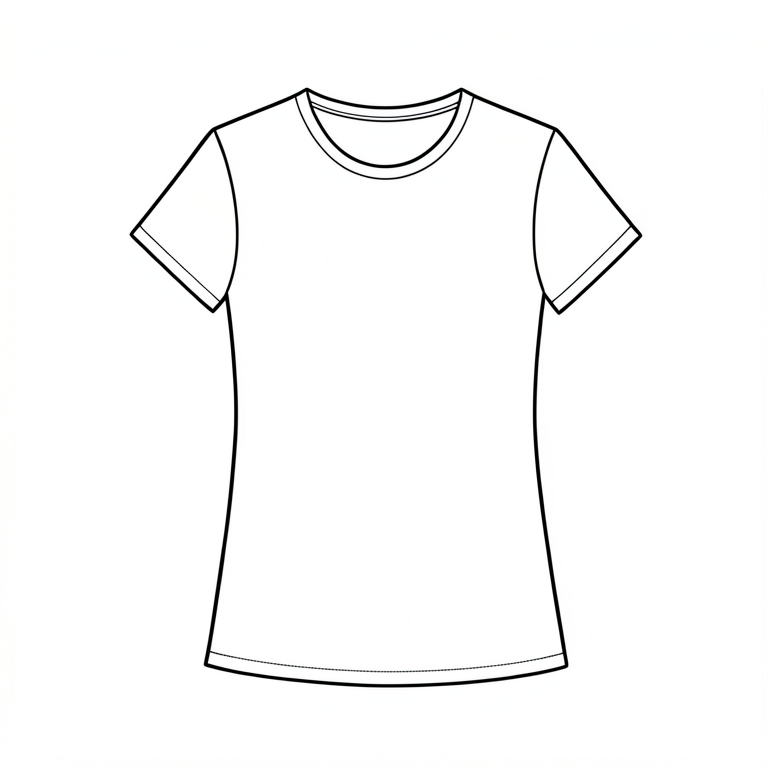
\includegraphics[width=0.36\linewidth]{img/base-top.png}
\caption{A base sketch from the first test run: a plain top drawn from the style sentence alone. Neckline and sleeve options are edits of a sketch like this one.}
\label{fig:base}
\end{figure}

\section{Ranking, review and cleaning}
Each option is drawn from two seeds: by editing its base where it has one, so the set stays consistent, and from text otherwise. CLIP ViT-L/14 \cite{radford2021clip} scores every variant against the descriptions of all options in its group, so a variant scores well only if it shows this option and not a neighbouring one; a sweetheart neckline that CLIP mistakes for a square one is ranked down. Line drawings that touch the edge of the frame or are mostly dark are penalised. Generators often draw necklines and sleeves wrongly, so the ranking is a first pass only: contact sheets of every option with its variants are reviewed by hand, and the choices are recorded in a file that the publishing step reads before it falls back to the ranking.

Publishing turns each sketch into ink on a transparent background (white becomes transparent, lines keep their weight), trims and centres it, and saves it as a 384\,px WebP; photographs are cropped square. The manifest maps each key to its file. A test checks that every file exists and is under 80\,kB, that every key is an ontology value, and that every question the assistant can ask, for every garment and season, can be answered by picture.

\section{Status}
The pipeline, the catalogue, the interface and the tests are complete, and the first base sketches show the intended style (Figure~\ref{fig:base}). The full library of 171 pictures is being generated and reviewed; until it is published, the interface falls back to the text choices it used before, option by option.

\chapter{The application}\label{ch:app}

\section{Interface}
The interface follows two rules: the customer should always be able to read what the system understood, and nothing should look different from everything else. Type is Inter for the interface and Bodoni Moda for headlines, on white. Every control is a rounded pill or card from one set of shapes; the views are switched by a segmented control; editing a detail opens a sheet that slides up over the page. The home page (Figure~\ref{fig:home}) says what the service does and starts a design. Its centrepiece is a sphere rendered live on the GPU by a fragment shader (noise-displaced surface, specular highlight, thin-film iridescence at grazing angles) that breathes when idle and ripples with the voice level while the customer speaks; without WebGL it falls back to a still image of the same look.

\begin{figure}[tbp]
\centering
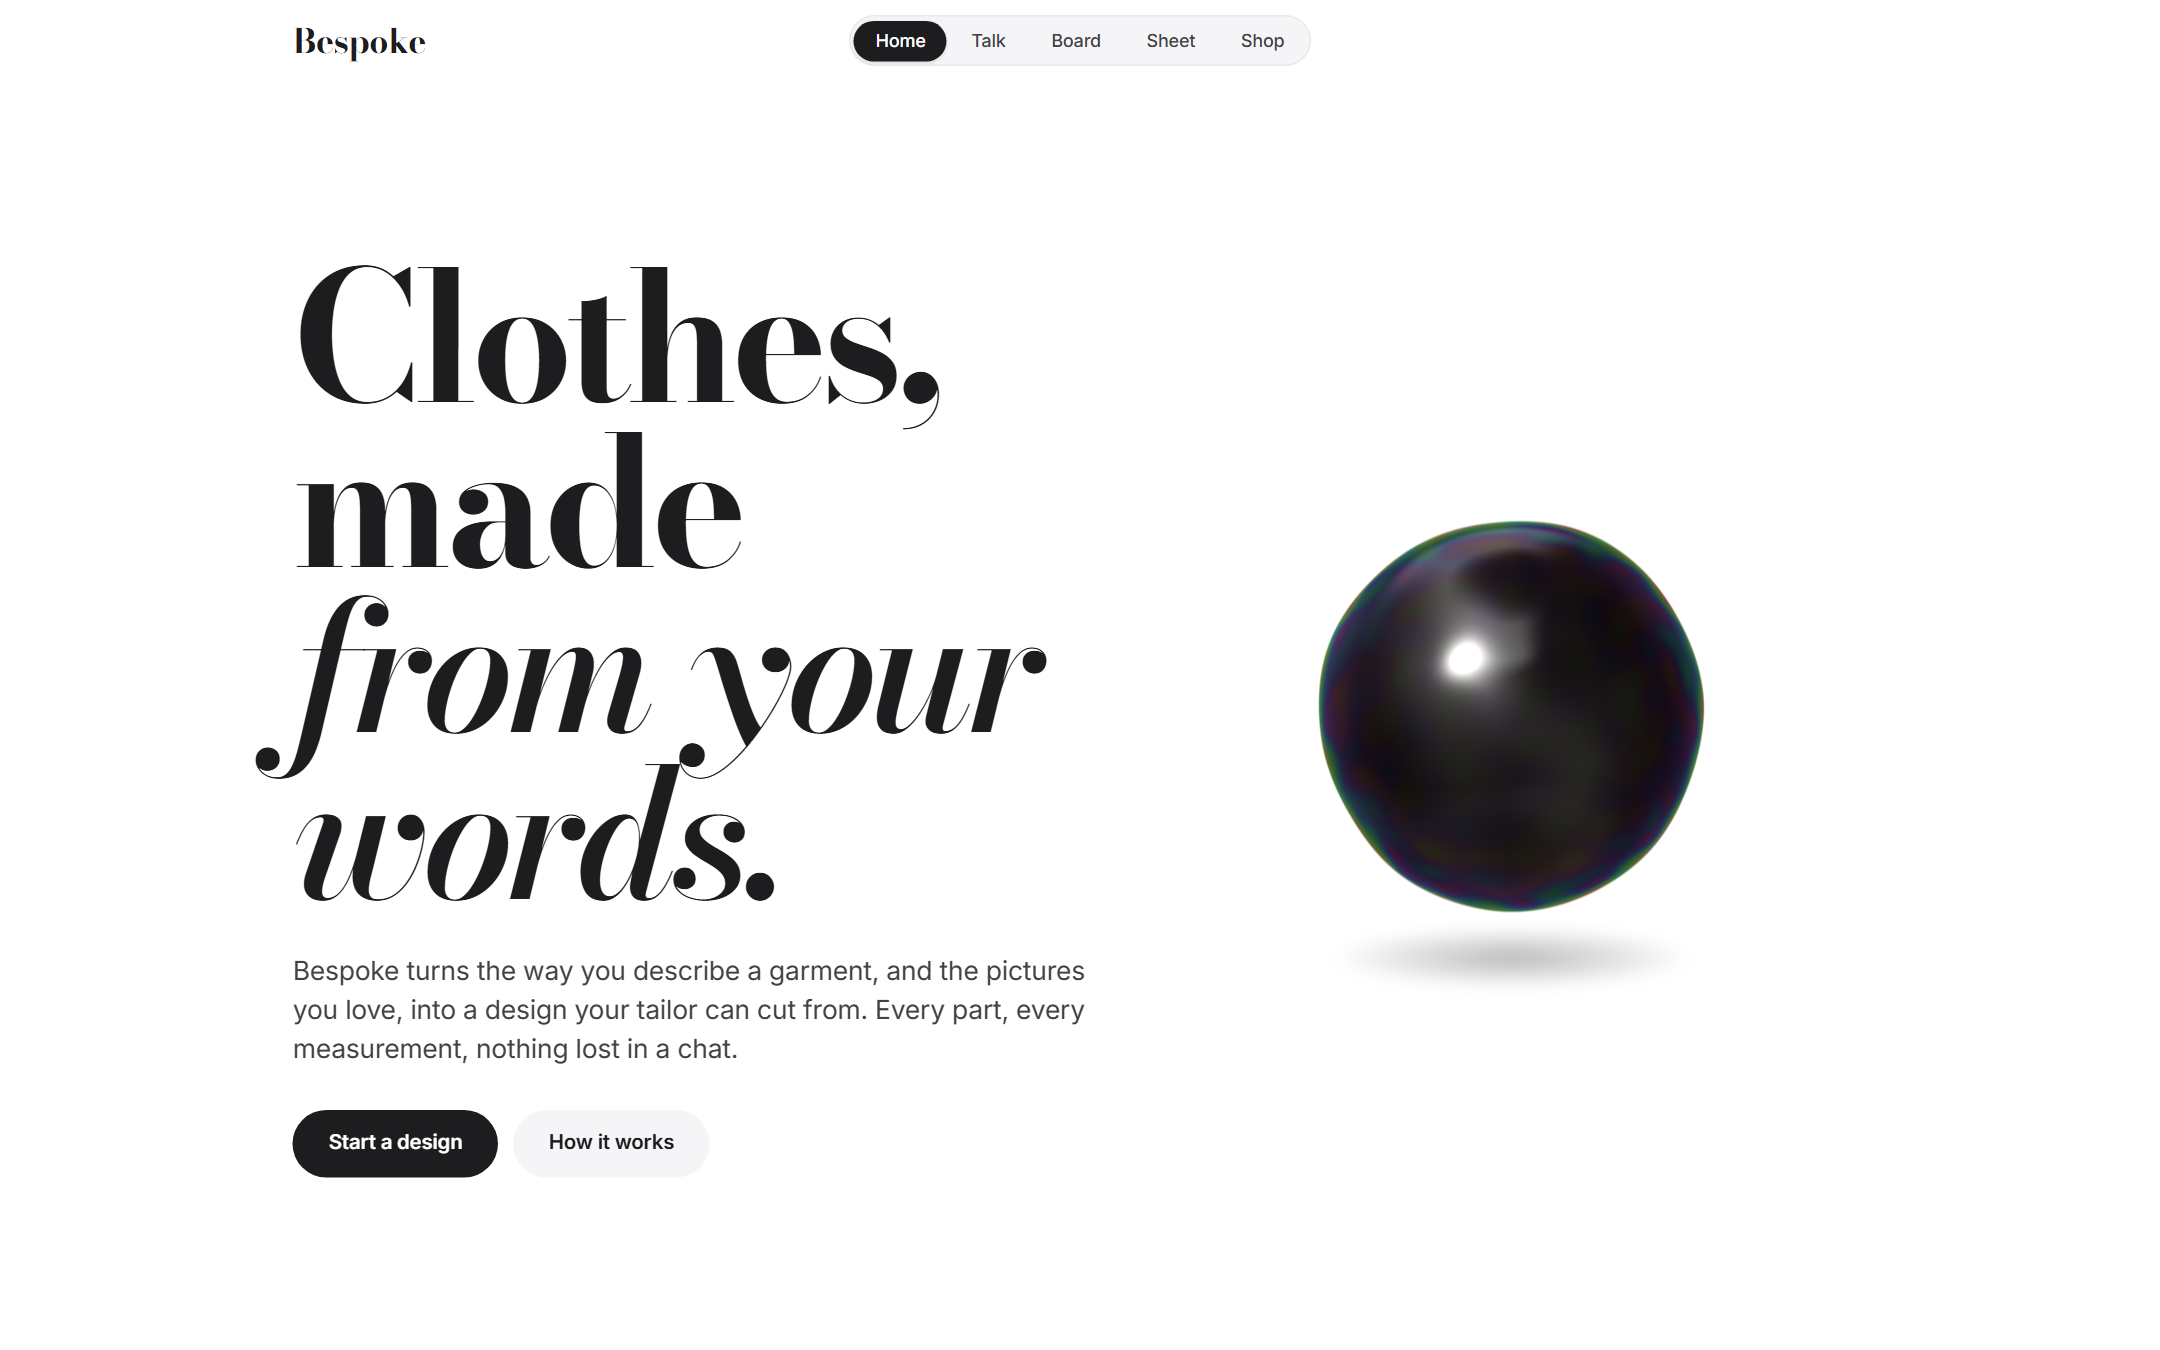
\includegraphics[width=\linewidth]{img/home.png}
\caption{The home page at desktop width.}
\label{fig:home}
\end{figure}

\section{The conversation}
The conversation view (Figure~\ref{fig:talk}) answers in one sentence, shows the request with the understood words underlined, and lists the design on an order card: each row a slot, its value, and where it came from. Any row can be changed by tapping it, which opens a picker; for colour the picker is a palette with a shade maker that records the exact shade as a note for the tailor. At most two questions are asked per turn. Every step can be taken back: before each message, answer, edit or board reading the design and the conversation are saved, and a Back button under the latest reply restores the previous state exactly, up to thirty steps. When the design is complete, the tailor sheet and the shopping links appear in the conversation itself, so the customer is not sent elsewhere to finish.

\begin{figure}[tbp]
\centering
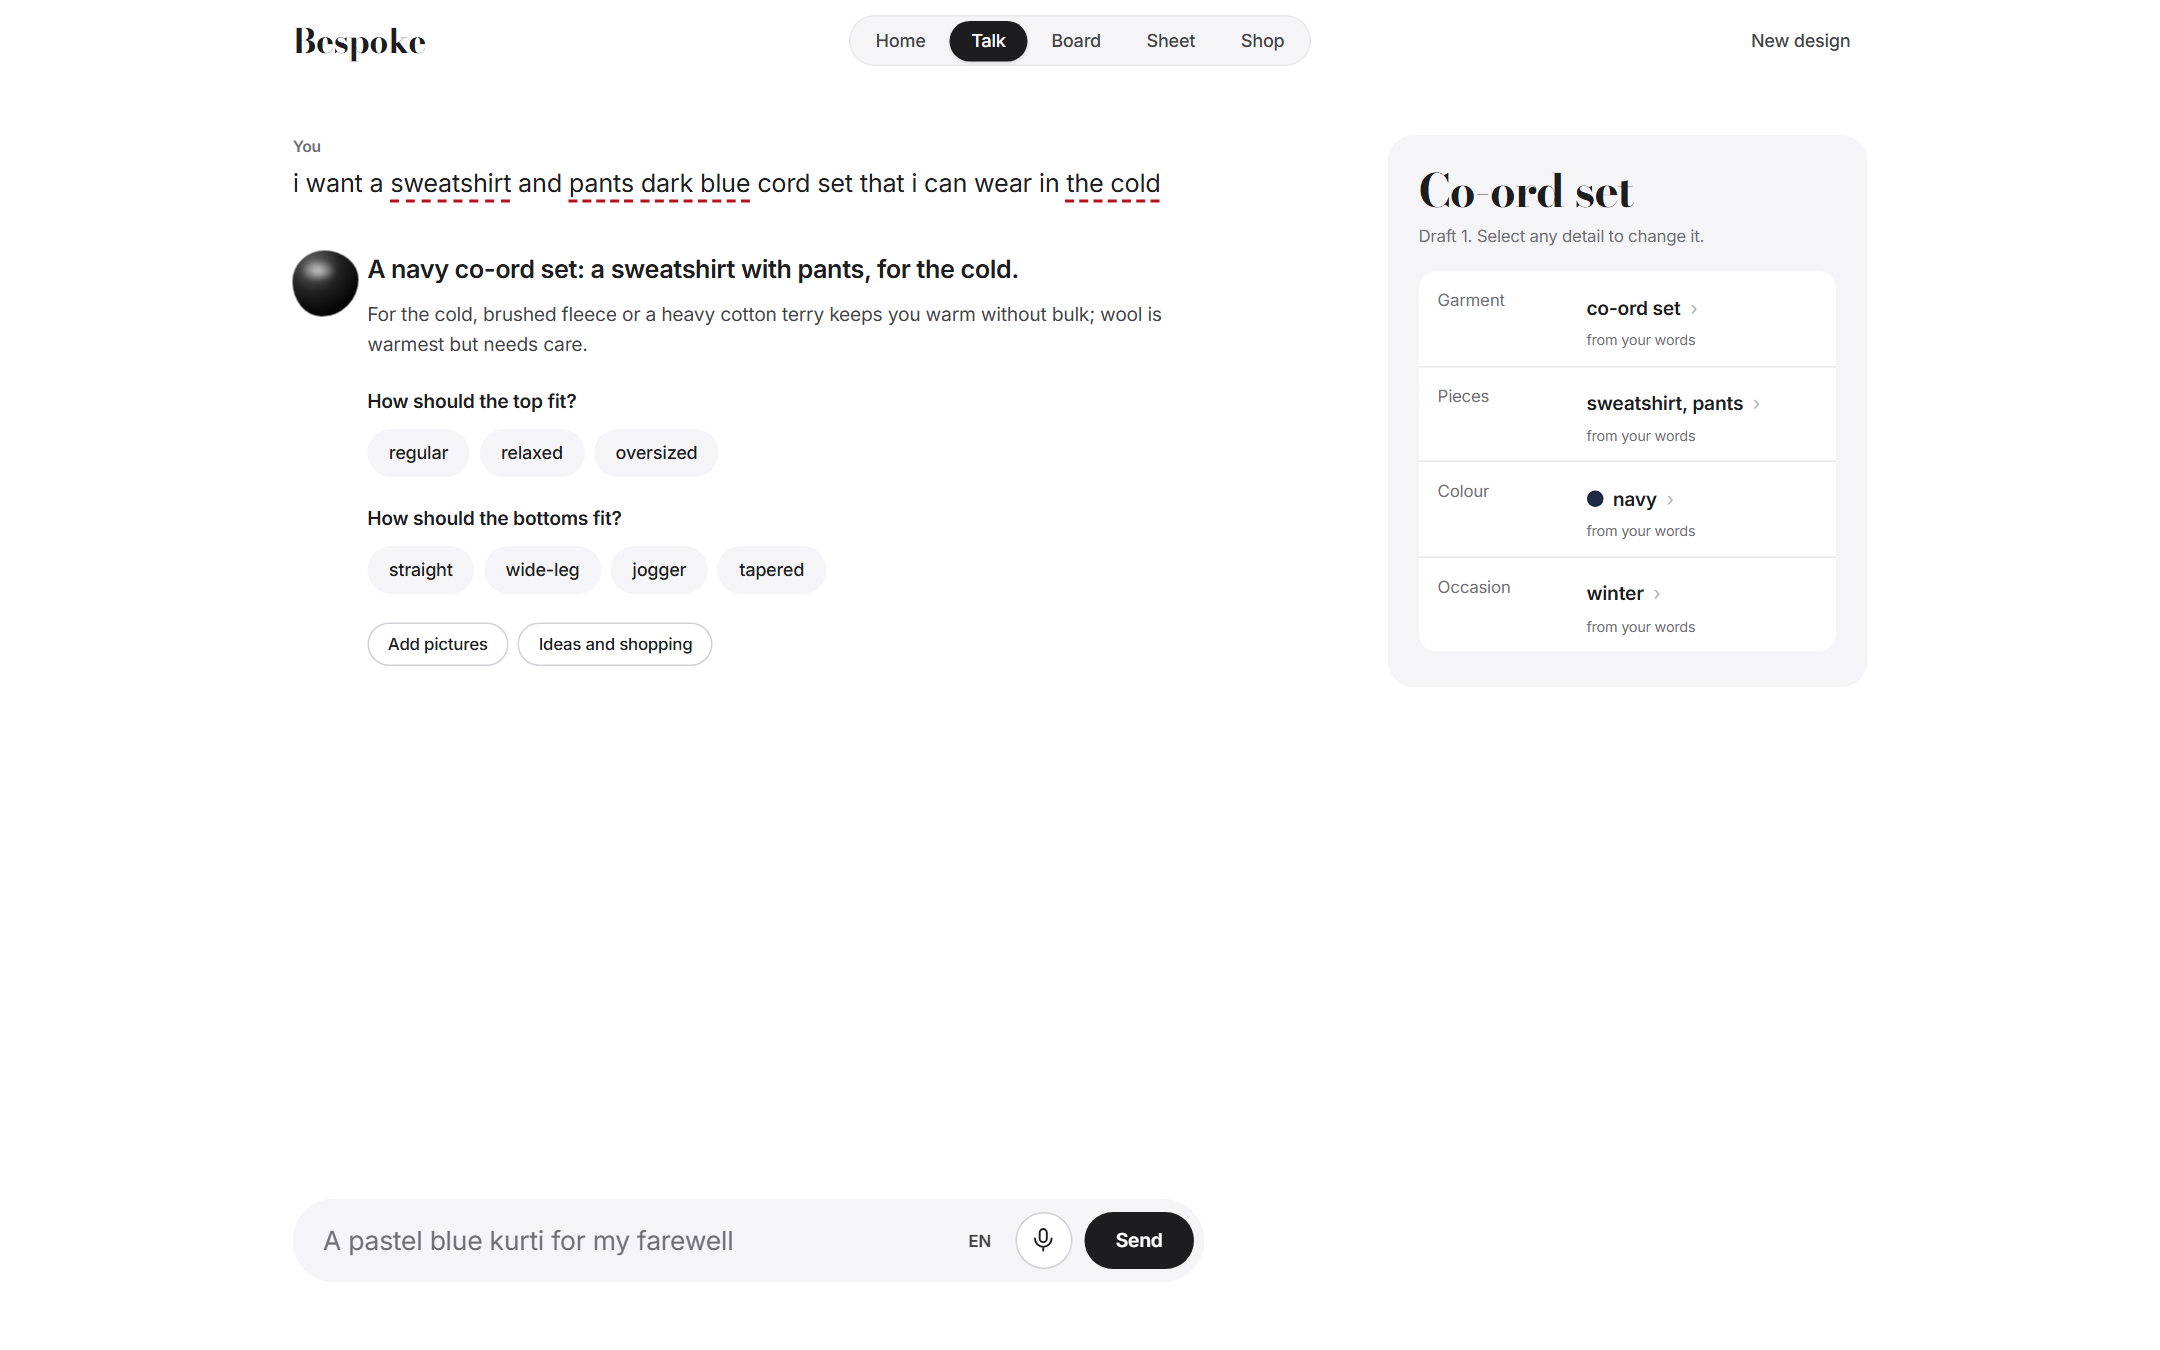
\includegraphics[width=\linewidth]{img/talk.png}
\caption{The request that the first version misread, now a navy co-ord set for winter. The questions are about fit and warm fabrics; there is no neckline question for a sweatshirt.}
\label{fig:talk}
\end{figure}

\section{The moodboard}
The board is an embedded Excalidraw canvas \cite{excalidraw}, used under its MIT licence, with its own menu and the licence notice kept in the site's open-source notices. Customers drop or paste pictures, write notes, draw arrows from a note to the picture it describes and circle the part they like. Reading the board numbers the pictures and scores each one with CLIP zero-shot \cite{radford2021clip}, on the device. Only garment, colour and print are read from a whole picture, because zero-shot scores for necklines and sleeves on unconstrained photos proved unreliable; those are read only from circled regions. A value from pictures is used only if its probability is at least 0.55 and leads the next by 0.2, and its confidence is capped at 0.6, so it can fill a gap but never overrule what the customer wrote.

\section{The tailor sheet}
The sheet (Figure~\ref{fig:sheet}) lists every instruction by part with its source, so the tailor can tell the customer's words from a default. It switches wholly to Hindi, including part names, values, labels and the finished measurements, which are the customer's body measurements plus the ease the fit implies. Drawings of the chosen neckline, sleeves, shape, length and fabric are printed beside the instructions once the picture library is published. The sheet prints to A4 or saves as PDF.

\begin{figure}[tbp]
\centering
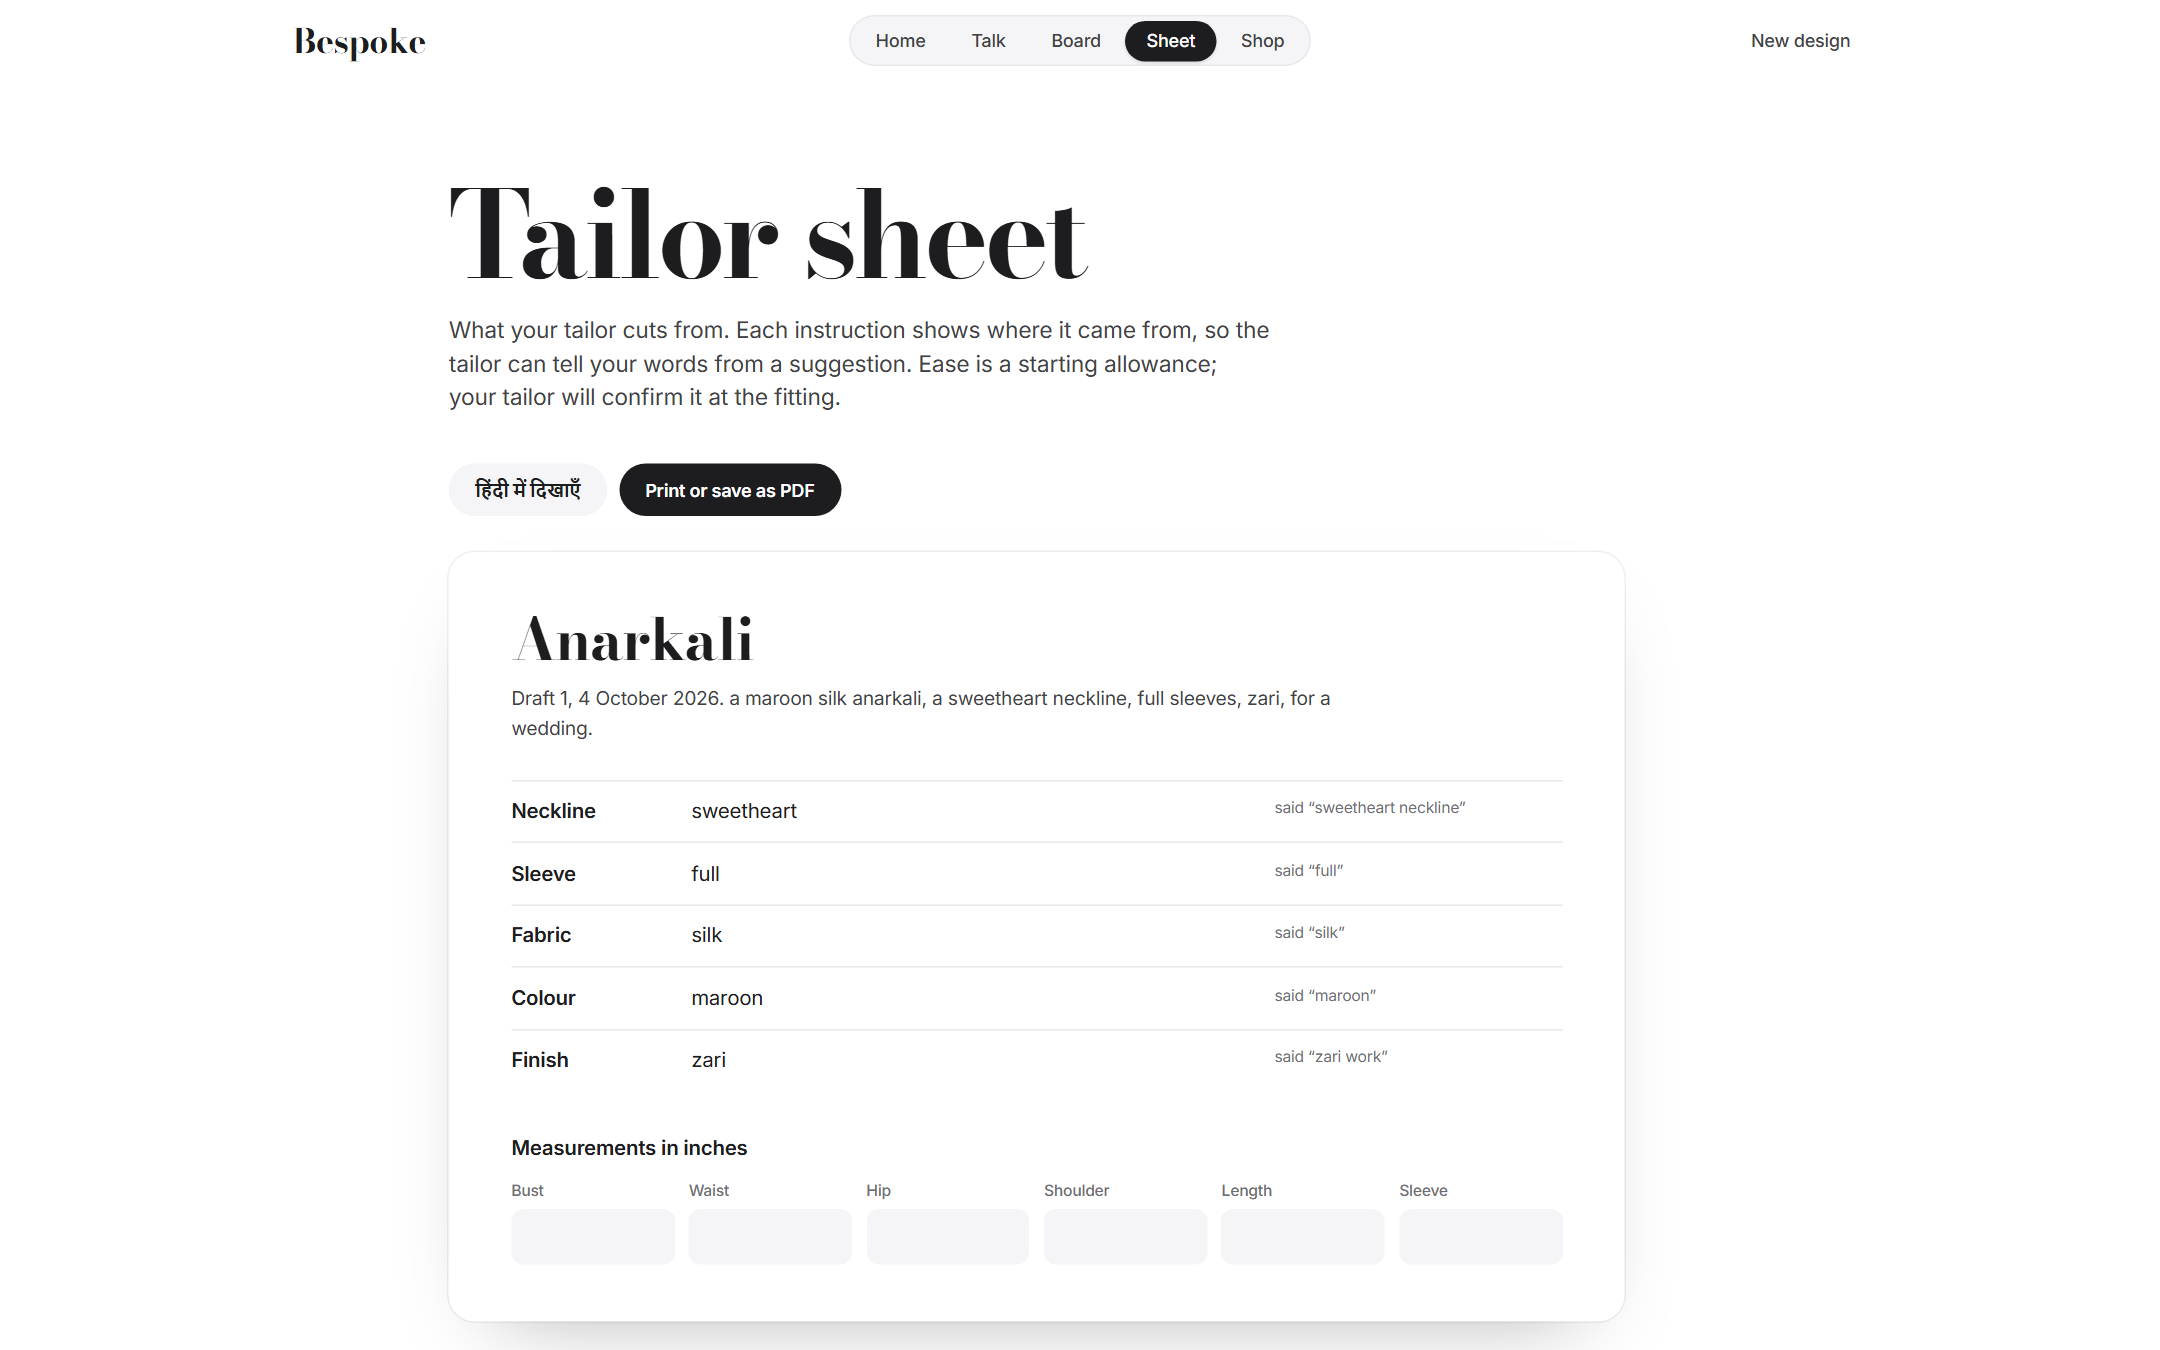
\includegraphics[width=0.49\linewidth]{img/sheet.png}\hfill
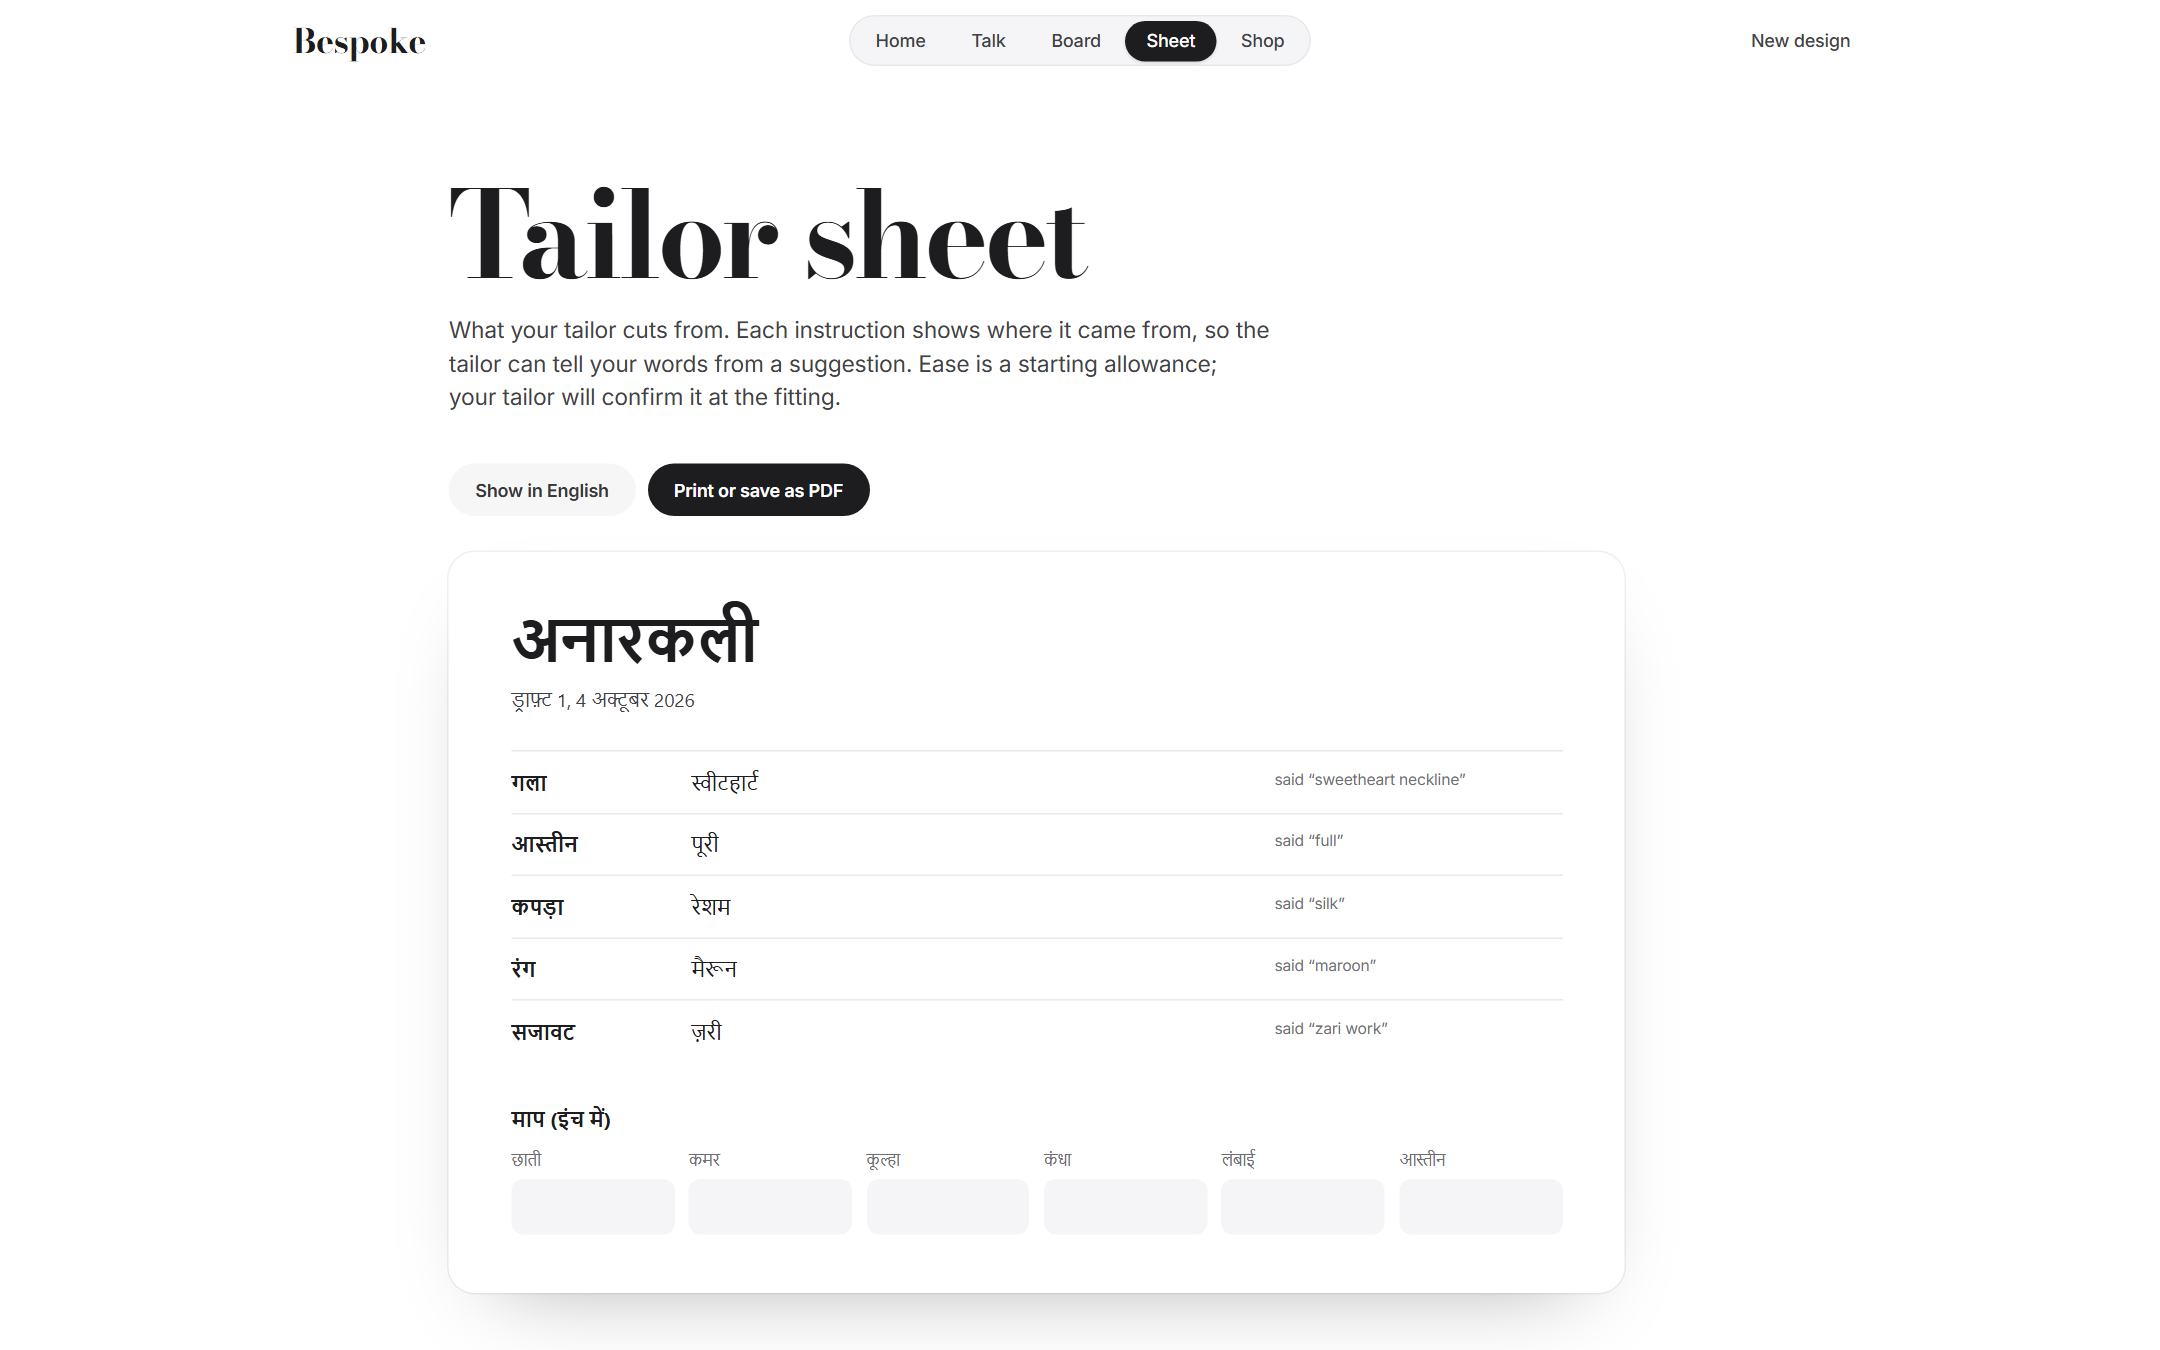
\includegraphics[width=0.49\linewidth]{img/sheet-hi.png}
\caption{The same tailor sheet in English and in Hindi.}
\label{fig:sheet}
\end{figure}

\section{Shopping and ideas}
The shop view writes one search from the design and opens it on Myntra, Ajio, Amazon, Flipkart and Nykaa Fashion, with Pinterest searches for ideas, fabric by the metre and tailors nearby on a map. Searches for garments worn by everyone are prefixed with the wearer, which the binder infers from the request and the customer can switch between women, men and anyone. Pinterest content is linked, not copied: its terms forbid storing pins or training on them.

\section{Deployment}
The site is a static export of a Next.js application, deployed on Vercel from the public repository \code{riteshroshann/onestyle}, with one serverless function for the optional model layer. The model key is held only in the host's environment. With no key the site is complete; the function answers 501 and the page uses the engine alone. The site works on phones, where the navigation stacks under the brand and every control is at least 32 pixels tall (Figure~\ref{fig:phone}).

\begin{figure}[tbp]
\centering
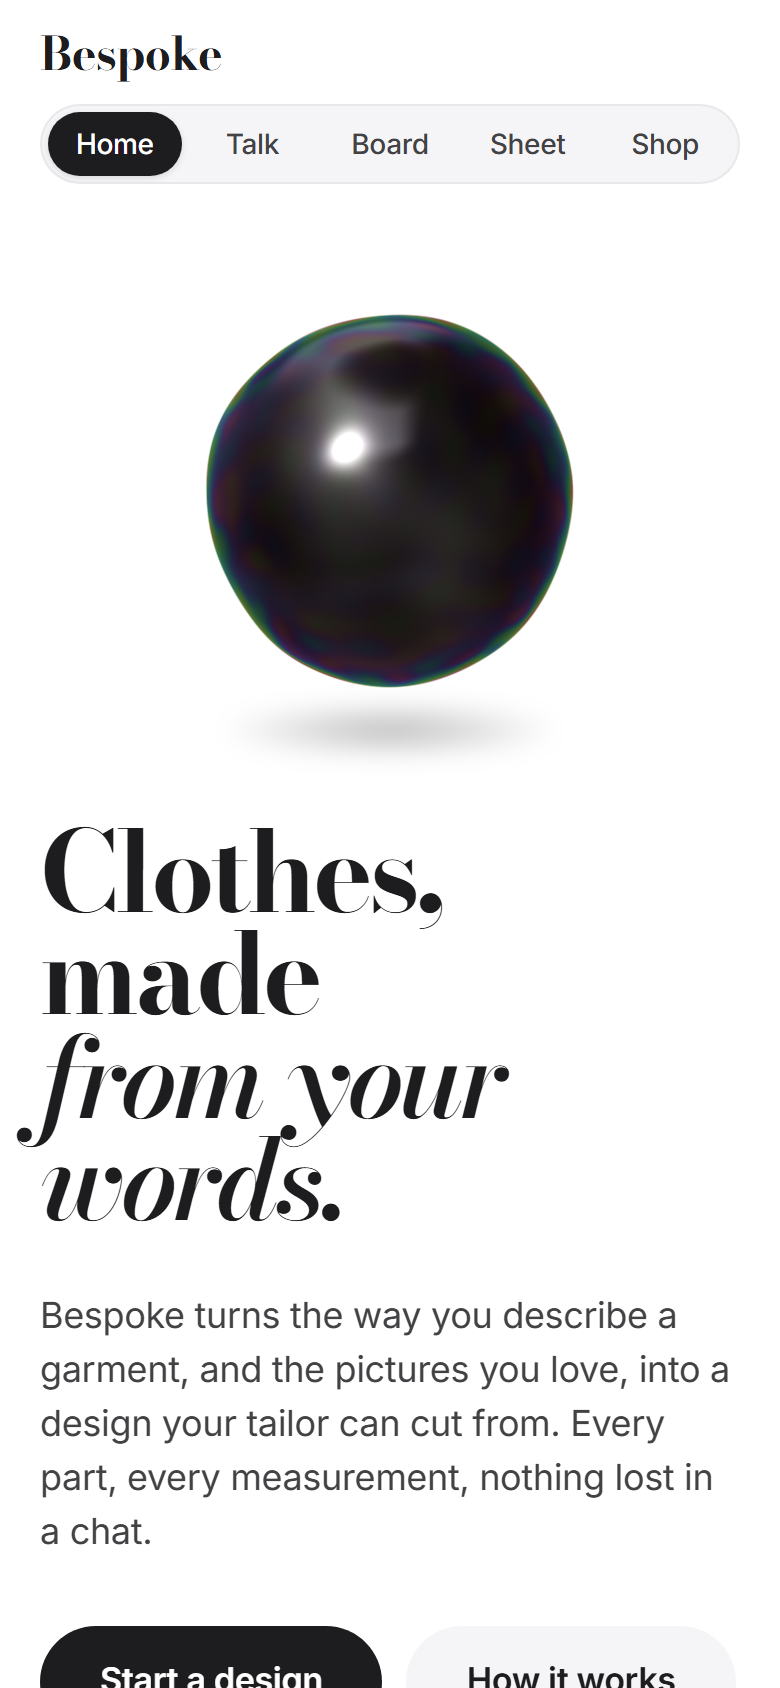
\includegraphics[width=0.3\linewidth]{img/phone.png}
\caption{The home page on a 390-pixel phone.}
\label{fig:phone}
\end{figure}

\chapter{Testing and measurement}\label{ch:tests}

\section{What is tested}
Seven kinds of test run locally before every release (Table~\ref{tab:tests}). Node runs the engine suites directly on the TypeScript sources; pytest runs the engine and model tests; and Playwright drives a real Chromium against the production build, with a server that behaves like a deployment without a model key.

\begin{table}[tbp]
\centering
\small
\begin{tabularx}{\linewidth}{@{}P{2.7cm}P{4.1cm}L@{}}
\thd{kind} & \thd{where} & \thd{what it holds the system to}\\\gap
unit & 34 engine tests; 14 Python tests & tokeniser, gazetteer, decoding, binding, the fold, questions, links\\
regression & 352 parity fixtures; F1 floor & the browser engine matches Python on every fixture; deployed F1 stays at or above 0.93; ONNX within 0.03 of PyTorch\\
functional & 21 realistic requests; browser flows & sets, seasons, wearers, editing, contradictions, the Hindi sheet, the picture picker\\
integration & model layer; tagger with the page & validation of model output, timeouts and errors fall back; tagger, engine and interface together\\
smoke & every view; shipped files & the build serves, each view opens, the model files are present, no console errors\\
usability & axe-core audits; phone & WCAG 2 AA with no serious findings, keyboard-only use, touch targets, no sideways scrolling, reduced motion\\
negative and edge & 22 engine cases; browser & empty, 20,000-character, emoji, Devanagari, gibberish and contradictory input; markup; double send; blocked storage; model CDN unreachable\\
\end{tabularx}
\caption{The test suite. All suites pass on the released build.}
\label{tab:tests}
\end{table}

\section{Accuracy}
Table~\ref{tab:f1} gives precision, recall and F1 for each tagger on the 52 test requests. The deployed combination is best on all three measures. The interval of the rules alone overlaps it, which is expected on a test set this size; the plan's benchmark of 1,200 requests, 40\% Hinglish and labelled by two annotators, is what will separate them.

\begin{table}[tbp]
\centering
\small
\begin{tabularx}{0.92\linewidth}{@{}Lrrrr@{}}
\thd{system} & \thd{precision} & \thd{recall} & \thd{F1} & \thd{95\% interval}\\\gap
HMM & 0.792 & 0.714 & 0.751 & 0.693--0.809\\
MiniLM alone & 0.842 & 0.784 & 0.812 & 0.754--0.866\\
CRF & 0.881 & 0.788 & 0.832 & 0.789--0.876\\
CRF with gazetteer features & 0.919 & 0.882 & 0.900 & 0.853--0.942\\
rules and gazetteer & 0.953 & 0.918 & 0.936 & 0.898--0.967\\
\textbf{MiniLM with gazetteer} & \textbf{0.955} & \textbf{0.951} & \textbf{0.953} & 0.918--0.982\\
\end{tabularx}
\caption{Span-level scores on held-out hand-written requests.}
\label{tab:f1}
\end{table}

\section{Speed}
Latency was measured on the development laptop (Table~\ref{tab:lat}). The engine itself is negligible; the tagger dominates, and the whole round trip from pressing send to the answer on screen is under a tenth of a second at the median. The only slow moment is the first visit, when the 33.8\,MB tagger downloads; the page answers from the gazetteer alone until it arrives.

\begin{table}[tbp]
\centering
\small
\begin{tabularx}{0.8\linewidth}{@{}Lrr@{}}
\thd{step} & \thd{median} & \thd{95th percentile}\\\gap
engine, one request after tagging & 0.04\,ms & 0.09\,ms\\
int8 tagger, ONNX Runtime, one thread & 3.6\,ms & 7.0\,ms\\
tagger in the browser, WebAssembly & 20\,ms & 53\,ms\\
send to answer on screen & 75\,ms & 130\,ms\\
first contentful paint & 340\,ms & \\
tagger first load, empty cache & 3.4\,s & \\
\end{tabularx}
\caption{Latency on a laptop CPU, with no GPU used for the tagger.}
\label{tab:lat}
\end{table}

\chapter{Phases}\label{ch:phases}

The work is organised in six phases, each with an exit test that decides when it is done (Figure~\ref{fig:roadmap}). Phases 0, 1 and 3 are complete and the application is live. Phase 2 is built: the board reader is deployed and the picture pipeline, catalogue, interface and tests are finished, with the library itself being generated. Phases 4 and 5 are planned and are where the Big Data Analytics half of the course is applied at scale.

\begin{figure}[tbp]
\centering
\resizebox{\linewidth}{!}{\begin{tikzpicture}[x=1cm,y=1cm,
  ttl/.style={font=\normalsize,anchor=base,text width=3.0cm,align=center},
  ph/.style={font=\small\scshape,anchor=base},
  pill/.style={rounded corners=4pt,inner xsep=5pt,inner ysep=2pt,font=\scriptsize\scshape,text=white},
  st/.style={box,text width=2.75cm,font=\small,inner ysep=5pt,minimum height=1.25cm},
  ex/.style={font=\footnotesize,text width=2.95cm,align=left,text=soft,anchor=north}]
\def\dx{3.32}
\draw[draw=greyD,line width=0.9pt] (-0.6,0) -- (5*\dx+0.6,0);
\foreach \i/\c/\t/\p/\s/\pc/\fl/\dr/\a/\b/\cc/\e in {
 0/ph0/{Environment\\and data}/Phase 0/done/greenT/sandF/sandD/{ontology: 1,212 forms, 47 garments}/{12,000 weak labels; 82 hand-written requests}/{Python and browser engines, 352 parity fixtures}/{both engines agree on every fixture.},
 1/ph1/{Language\\engine}/Phase 1/done/greenT/blueF/blueD/{rules, HMM, CRF, MiniLM on one split}/{constrained Viterbi; int8 ONNX, 33.8\,MB}/{binder, fold, question policy, voice}/{F1 0.953 on held-out requests; 75\,ms per turn.},
 2/ph2/{Pictures and\\moodboard}/Phase 2/{built, library in progress}/sandT/lavF/lavD/{board reading with CLIP, words outrank pictures}/{FLUX.2 [klein] on a 6\,GB GPU}/{CLIP ranking, review, 171 static pictures}/{every question answerable by picture.},
 3/ph3/{Studio and\\deployment}/Phase 3/live/greenT/roseF/roseD/{Talk, Board, Sheet, Shop, Home}/{Hindi sheet; model layer behind a key}/{seven kinds of test; Vercel}/{all suites pass on the released build.},
 4/ph4/{Data\\platform}/Phase 4/planned/greyT/greenF/greenD/{lake of orders and public retail data}/{Spark DataFrame jobs and their DAGs}/{MLlib: trends, ALS, FP-Growth}/{suggestions beat popularity on held-out orders.},
 5/ph5/{Tailors and\\benchmark}/Phase 5/planned/greyT/greyF/greyD/{1,200-request benchmark, 40\% Hinglish}/{study with practising tailors}/{paper and course report}/{tailors cut from the sheet without calling.}}{
  \node[ttl] at (\i*\dx,2.15) {\t};
  \node[ph,text=\c] at (\i*\dx,0.55) {\p};
  \path[fill=\c] (\i*\dx,0) circle (3.4pt);
  \node[pill,fill=\pc] at (\i*\dx,-0.62) {\s};
  \node[st,fill=\fl,draw=\dr] (a\i) at (\i*\dx,-1.95) {\a};
  \node[st,fill=\fl,draw=\dr] (b\i) at (\i*\dx,-3.6) {\b};
  \node[st,fill=\fl,draw=\dr] (c\i) at (\i*\dx,-5.25) {\cc};
  \draw[flow] (a\i) -- (b\i); \draw[flow] (b\i) -- (c\i);
  \node[ex] at (\i*\dx,-6.12) {\textit{Exit:} \e};
}
\end{tikzpicture}
}
\caption{The phases, their state as of October 2026, and the test each must pass.}
\label{fig:roadmap}
\end{figure}

\section{System across the phases}
Figure~\ref{fig:across} places each component in its phase. Solid blocks are built and deployed; dashed blocks are planned. The planned blocks attach to the outputs that exist today: the data platform will learn from the designs and answers the application already records, and the tailor study will test the sheet the application already prints.

\begin{figure}[tbp]
\centering
\resizebox{\linewidth}{!}{\begin{tikzpicture}[x=1cm,y=1cm,
  b/.style={box,minimum height=1.55cm,text width=1.75cm,font=\small},
  br/.style={decorate,decoration={brace,mirror,amplitude=5pt},line width=0.6pt},
  bl/.style={font=\small,anchor=north}]
\node[blue,b] (w) at (0,0.95) {words\\{\scriptsize\color{soft}typed, spoken}};
\node[peach,b] (p) at (0,-0.95) {board\\{\scriptsize\color{soft}pictures, notes}};
\node[blue,b] (tg) at (2.7,0.95) {tagger\\{\scriptsize\color{soft}rules + MiniLM}};
\node[peach,b] (cl) at (2.7,-0.95) {CLIP\\{\scriptsize\color{soft}pooled}};
\node[lav,b,minimum height=3.45cm] (bd) at (5.3,0) {binder\\{\scriptsize\color{soft}parts, sets, seasons}};
\node[green,b,minimum height=3.45cm] (sp) at (7.9,0) {Design\-Spec\\{\scriptsize\color{soft}a fold of updates}};
\node[sand,b] (q) at (10.5,0.95) {questions\\{\scriptsize\color{soft}by picture}};
\node[rose,b] (sh) at (10.5,-0.95) {tailor sheet\\{\scriptsize\color{soft}English, Hindi}};
\node[green,b,planned] (ml) at (13.1,0.95) {Spark\\{\scriptsize\color{soft}trends, ALS}};
\node[grey,b,planned] (tl) at (13.1,-0.95) {tailors\\{\scriptsize\color{soft}study, feedback}};
\draw[flow] (w) -- (tg); \draw[flow] (p) -- (cl);
\draw[flow] (tg) -- (tg-|bd.west); \draw[flow] (cl) -- (cl-|bd.west);
\draw[flow] (bd) -- (sp);
\draw[flow] (sp.east|-q) -- (q); \draw[flow] (sp.east|-sh) -- (sh);
\draw[dflow] (q) -- (ml); \draw[dflow] (sh) -- (tl);
\draw[flow] (q.north) -- ++(0,0.45) -| node[pos=0.25,above,font=\scriptsize,text=soft]{answers fold back into the design} (sp.north);
\draw[br,draw=ph1] (1.75,-1.95) -- (6.25,-1.95) node[bl,midway,below=5pt,text=ph1] {Phases 1, 2};
\draw[br,draw=ph3] (6.95,-1.95) -- (11.45,-1.95) node[bl,midway,below=5pt,text=ph3] {Phases 2, 3};
\draw[br,draw=ph4] (12.15,-1.95) -- (14.05,-1.95) node[bl,midway,below=5pt,text=ph4] {Phases 4, 5};
\end{tikzpicture}
}
\caption{The components and the phases that build them. Solid blocks exist and are tested; dashed blocks are planned.}
\label{fig:across}
\end{figure}

\section{Phase 4: the data platform}
The research plan specifies the platform in detail. Designs, answers and orders are written as events to a lake of Parquet files partitioned by day, alongside the public H\&M and Amazon fashion datasets. Spark jobs written with DataFrames clean and join them, and their execution plans are kept as evidence of how the work is divided across executors. MLlib pipelines learn what the application cannot learn from one customer: TF-IDF and Word2Vec over request text to find new surface forms for the ontology, FP-Growth over completed designs to find attribute combinations that go together, and ALS over customers and attributes to suggest fabrics and colours. The exit test is that suggestions beat a popularity baseline on held-out orders.

\section{Phase 5: tailors and the benchmark}
The test set is 52 requests written by the developer. Phase 5 replaces it with \textsc{bespoke-spec}: 1,200 requests, 40\% in Hinglish, labelled by two annotators with agreement measured. The other half of the phase is a study with practising tailors, who receive tailor sheets for real orders. The exit test is the one that matters for the product: a tailor cuts the garment from the sheet without phoning the customer.

\chapter{Limits and conclusion}\label{ch:end}

\section{Limits}
\paragraph{The test set is small} Fifty-two requests give intervals about seven points wide. The ranking of the deployed tagger over the HMM and CRF is clear; its lead over the rules alone is not yet significant.

\paragraph{The training data is synthetic} Templates and catalogue titles do not sound like customers. The gazetteer covers for this today. Real requests from the application, with consent, are the remedy, and the plan's benchmark is the measure.

\paragraph{Pictures are read coarsely} Zero-shot CLIP is reliable for garment type, colour and print on whole pictures, and not for necklines or sleeves. Attribute heads trained on fashion images, as the plan proposes with FashionSigLIP, are needed before the board can read fine detail.

\paragraph{Generated pictures can be wrong} Image models draw necklines and sleeves wrongly often enough that every published picture is reviewed by hand. The ranking narrows the choice; it does not replace the review.

\paragraph{Ease values are defaults} The allowance added for each fit is a starting value, marked as such on the sheet. Partner tailors' own values will replace it.

\section{Conclusion}
Bespoke shows that the gap between a customer's loose, mixed-language description and an instruction a tailor can cut from can be closed with a small, careful system that runs in the browser. The ontology carries the domain knowledge; a gazetteer and a fine-tuned 33-million-parameter encoder together tag requests with F1 0.953; a binder and a fold turn spans into a design whose every value has a source; and a question policy asks only what a tailor needs, in the order that matters. A language model is used where it helps and is never trusted unchecked. Choices are made by looking, from pictures made on a laptop with an open model. The application is live, tested and fast. What remains is scale: the data platform that learns from orders, and the tailors who will judge whether the sheet is enough.


\backmatter
\begingroup
\small
\renewcommand{\bibname}{References}
\begin{thebibliography}{99}
\addcontentsline{toc}{chapter}{References}
\setlength{\itemsep}{3pt}

\bibitem{aggarwal2019myntra} P.~Aggarwal. Fashion Product Images Dataset (Myntra catalogue, 44,446 items). Kaggle, 2019.

\bibitem{bfl2024flux} Black Forest Labs. Announcing Black Forest Labs: FLUX.1 [schnell], released under Apache 2.0. bfl.ai, 1 August 2024.

\bibitem{bfl2026klein} Black Forest Labs. FLUX.2 [klein]: towards interactive visual intelligence. Model card and weights, huggingface.co/black-forest-labs/FLUX.2-klein-4B, Apache 2.0, 2026.

\bibitem{bian2025chatgarment} S.~Bian et al. ChatGarment: garment estimation, generation and editing via large language models. \emph{CVPR}, 2025, pp.~2924--2934. doi:10.1109/CVPR52734.2025.00278.

\bibitem{cheng2026chatpref} Y.~Cheng et al. ChatPreference: a large language model for customer preference understanding in the apparel industry. \emph{Journal of Engineering Design} 37(9), Taylor \& Francis, 2026, pp.~3560--3589. doi:10.1080/09544828.2026.2655935.

\bibitem{dataforindia} Data For India. The rise of custom tailoring (analysis of PLFS 2023--24). dataforindia.com, 2025.

\bibitem{devlin2019bert} J.~Devlin, M.-W.~Chang, K.~Lee, K.~Toutanova. BERT: pre-training of deep bidirectional transformers for language understanding. \emph{NAACL}, 2019.

\bibitem{excalidraw} Excalidraw contributors. Excalidraw: virtual whiteboard for sketching hand-drawn like diagrams. github.com/excalidraw/excalidraw, MIT licence.

\bibitem{hm2022} H\&M Group. H\&M Personalized Fashion Recommendations. Kaggle competition dataset, 2022.

\bibitem{jia2020fashionpedia} M.~Jia et al. Fashionpedia: ontology, segmentation, and an attribute localization dataset. \emph{ECCV}, Springer, 2020.

\bibitem{lafferty2001crf} J.~Lafferty, A.~McCallum, F.~Pereira. Conditional random fields: probabilistic models for segmenting and labeling sequence data. \emph{ICML}, 2001.

\bibitem{radford2021clip} A.~Radford et al. Learning transferable visual models from natural language supervision. \emph{ICML}, 2021.

\bibitem{radford2023whisper} A.~Radford et al. Robust speech recognition via large-scale weak supervision. \emph{ICML}, 2023.

\bibitem{wang2020minilm} W.~Wang et al. MiniLM: deep self-attention distillation for task-agnostic compression of pre-trained transformers. \emph{NeurIPS}, 2020.

\end{thebibliography}
\endgroup

\end{document}
